\subsection{3D->2D vetítési algoritmusok, a window-viewport transzformáció.}

\textbf{Képalkotás:}
\begin{itemize}
    \item térbeli modellek képernyőre (tér -> sík leképzés)
\end{itemize}

\begin{equation*}
    \xi = f_\xi(x, y, z)
\end{equation*}
\begin{equation*}
    \eta = f_\eta(x, y, z)
\end{equation*}

\textbf{Vetítés párhuzamos vetítősugarakkal axonometria:}
\begin{equation*}
    \xi = -x \cdot q_x \cdot \cos(\alpha) + y \cdot q_y \cdot \cos(\beta) - z \cdot q_z \cdot \sin(\gamma)
\end{equation*}
\begin{equation*}
    \eta = -x \cdot q_x \cdot \sin(\alpha) - y \cdot q_y \cdot \sin(\beta) + z \cdot q_z \cdot \cos(\gamma)
\end{equation*}

\begin{center}
    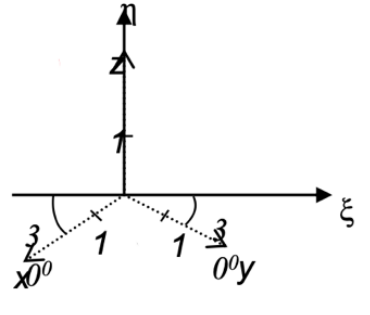
\includegraphics[width=0.6\textwidth]{res/imgs/info_21_axonometry.png}
\end{center}

\begin{itemize}
    \item \textbf{izometrikus axonometria:}
\end{itemize}
\begin{align*}
    q_x = 1, \quad q_y = 1, \quad q_z = 1 \\
    \alpha = 30^\circ, \quad \beta = 30^\circ, \quad \gamma = 0^\circ
\end{align*}

\begin{minipage}{0.4\textwidth}
    \begin{center}
        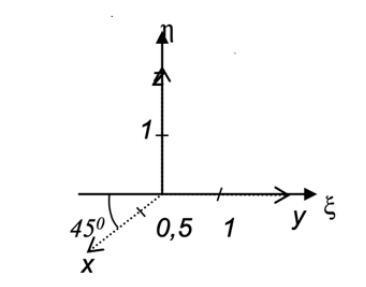
\includegraphics[width=\textwidth]{res/imgs/info_21_isometric.png}
    \end{center}
\end{minipage}
\hfill
\begin{minipage}{0.5\textwidth}
    \begin{align*}
        \xi &= -x \cdot \frac{\sqrt{3}}{2} + y \cdot \frac{\sqrt{3}}{2} \\
        \eta &= -x \cdot 1 \cdot \frac{1}{2} - y \cdot 1 \cdot \frac{1}{2} + z
    \end{align*}
\end{minipage}

\begin{itemize}
    \item cavalier axonometria:
\end{itemize}
\begin{align*}
    q_x = 0.5, \quad q_y = 1, \quad q_z = 1 \\
    \alpha = 45^\circ, \quad \beta = 0^\circ, \quad \gamma = 0^\circ
\end{align*}

\begin{minipage}{0.4\textwidth}
    \begin{center}
        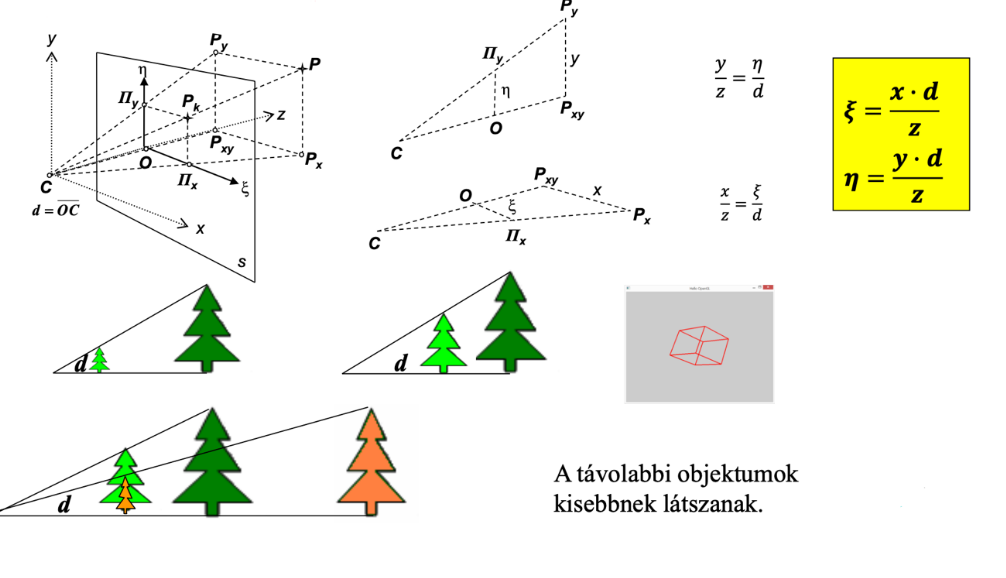
\includegraphics[width=\textwidth]{res/imgs/info_21_cavalier.png}
    \end{center}
\end{minipage}
\hfill
\begin{minipage}{0.5\textwidth}
    \begin{align*}
        \xi &= -0.5 \cdot x \cdot \frac{\sqrt{2}}{2} + y \\
        \eta &= -0.5 \cdot x \cdot \frac{\sqrt{2}}{2} + z
    \end{align*}
\end{minipage}

\textbf{Probléma:} azonos hosszú párhuzamos szakaszok azonos hosszúnak látszanak, nincs perspektíva, torzul a kép. A valós tárgyak torzítva jelennek meg, nincs térérzet.

\textbf{Centrális vetítés:}
\begin{center}
    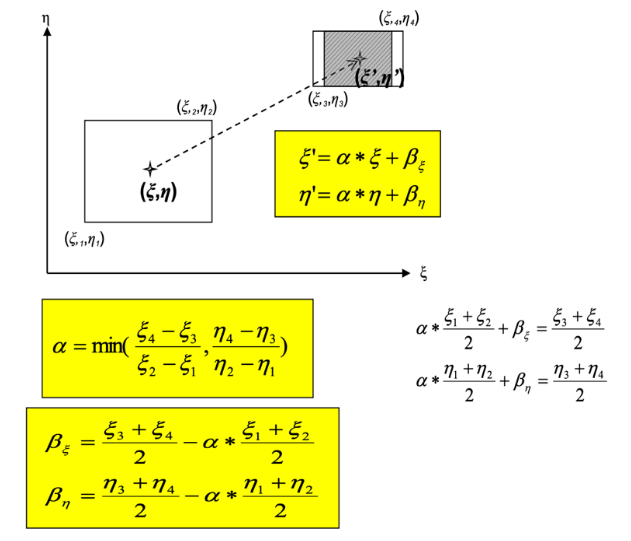
\includegraphics[width=0.9\textwidth]{res/imgs/info_21_central_projection.png}
\end{center}